\chapter{Endormissement de tache sous priorité Fixe}
\minitoc
\section{modéle de tâches}
Le modèle utilisé ici est le modèle de tâche périodique de Liu et
Layland défini au chapitre 1.\\ Soit $\taskset =
\{\task{1},\task{2},\cdots,\task{n}\}$ un ensemble de tache, chaque
tache $\task{i}$ est caracterisé par $\task{i} =
(\charge{i},\deadline{i},\period{i})$ et :
\begin{itemize}
\item $\task{i}$ est periodique.
\item $\charge{i}$ est le pire temps d'execution de la tache $i$.
\item $\deadline{i}$ est l'écheance relative de la tache $i$.
\item $\period{i}$ est la periode relative de la tache $i$.
\item l'ensemble de tâches $\taskset{}$ est ordonnançable avec
  l'algorithme Deadline Monotonic.
\end{itemize}
\section{Le cas monoprocesseur}
Dans cette section nous allons inserer une tâche d'endormissement
$\task{\sleep} = \{ \charge{\sleep}, \deadline{\sleep},
\period{\sleep}\}$ avec $\min \charge{\sleep} \leq \charge{\sleep}
\geq \max \charge{sleep}$ avec $\wcet{sleepMax} = (1-\util{}) \times
\period{H}$ et $\task{sleep} \cup \taskset{}$ est ordonnançable avec
Deadline Monotonic.


Pour cela nous presentons l'algorithme d'insertion de tache
d'endormissement $\task{\textsc{sleep}}$ dans un taskset $\taskset{}$.



%% refaire les algorithmes avec Algorithmics ! 
%\begin{algorithm}[H]
%\KwData{TaskSet $\taskset{}$, Temps Minimum d'execution
%  $\charge{SleepMin}$, Temps d'execution Maximum $\charge{SleepMax}$,
%  Pas de decrementation $\Delta \charge{}$} \KwResult{Tache
%  $\task{Sleep}$}
%\Begin{
% $\wcet{Sleep}  \longleftarrow \wcet{SleepMax}$ \;
% $\deadline{Sleep}	\longleftarrow \periode{H}$ \;
% $\periode{sleep} \longleftarrow \periode{H}$ \;
% \While{$\Gamma \cup tache(\wcet{Sleep},\deadline{Sleep},\periode{H})$ est non  ordonnançable et $\wcet{Sleep} \geq \wcet{SleepMin}$}
% {
% 	$\charge{\sleep} \longleftarrow \charge{\sleep} - \Delta \charge{}$ \;
% }
% $\task{\sleep} \longleftarrow CreerTache(\charge{\leep},\deadline{\leep},\period{\sleep})$
% }
% \caption{Insertion Taches Endormissement Dans Un Mono-processeur}
%\end{algorithm}









Nous illustrons notre algorithme avec un
exemple d'application. Le tableau \ref{tab:exempledmup} et la figure
\ref{fig:exempledmupapr} represente un ensemble de tâches $\taskset{}$
ordonnançable par Deadline Monotonic où on a inseré une tache
d'endormissement $\task{\textsc{sleep}}$:

\begin{table}[!h]
\begin{center}
\begin{tabular}{|c|c|c|c|}
 \hline$\task{i}$ & $\charge{i}$ & $\deadline{i}$ & $\period{i}$ \\ 
 \hline 1 & 1 & 10 & 10 \\ 
 \hline 2 & 2 & 15 & 15 \\ 
 \hline 
 \end{tabular}
\end{center}
\caption{Ensemble de t\^aches periodiques} \label{tab:exempledmup}
\end{table}

%\begin{figure}[h]
%\begin{center}
%\begin{RTGrid}[height=4cm,width=12cm,labelsize=8pt,numbersize=6]{3}{31}
%\multido{\n=0+10}{3}{
%\TaskArrDead{1}{\n}{10}}
%\TaskArrDead{1}{20}{10}

%\TaskExecution{1}{3}{4}
%\TaskExecution{1}{13}{14}
%\TaskExecution{1}{23}{24}

%\multido{\n=0+15}{2}{
%\TaskArrDead{2}{\n}{15}}
%\TaskArrDead{2}{15}{15}
%\TaskExecution{2}{4}{5}
%\TaskExecution{2}{8}{9}
%\TaskExecution{2}{18}{20}

%\multido{\n=0+5}{6}{
%\TaskArrDead{3}{\n}{5}}
%\TaskArrDead{3}{25}{5}
%\TaskExecution{3}{0}{3}
%\TaskExecution{3}{5}{8}
%\TaskExecution{3}{10}{13}
%\TaskExecution{3}{15}{18}
%\TaskExecution{3}{20}{23}
%\TaskExecution{3}{25}{28}

%\end{RTGrid}
%\caption{Insertion de tache dans un monoprocesseur} \label{fig:exempledmup}
%\end{center}
%\end{figure}

\section{Le cas multiprocesseur}
Dans cette section nous allons inserer un ensemble de tâches
d'endormissement
$\{\task{\sleep}^1,\task{\sleep}^2,...,\task{\sleep}^m\}$ tel que
$\task{\sleep}^i = \{ \charge{\sleep}^i, \deadline{\sleep}^i,
\period{\sleep}^i\}$ dans m processeurs $\proc{} =
\{\proc{1},\proc{2},...,\proc{m}\}$.  \indent Pour cela nous
presentons nous presentons deux strategie d'insertion :

\begin{description}
\item{Insertion Locale :} Chaque processeur$_i$ à sa propre tache
  d'endormissement $\task{\sleep}^i$
\item{Insertion Globale :} Tous les processeur ont une même tache
  d'endormissement
  $\task{\sleep}=\task{\sleep}^1=\task{\sleep}^2=...=\task{\sleep}^m$
\end{description}
Les deux algorithmes representent l'inseretion locale (Resp. globale)
d'un ensemble de tâches d'endormissement dans un ensemble de
processeur.


%\begin{center}
%\begin{algorithm}[H]
%\KwData{Ensemble de processeur $\proc{}$, Temps Minimum d'execution $\wcet{SleepMin}$}
%\KwResult{Ensemble de Tache d'endormissement $\taskset{Sleep}$}
%\Begin{
%	\For{$ \proc{i} \in \proc{}$}
%	{
%		$\tache{sleep}^i$ = tache\_endormissement\_monoprocesseur($\wcet{SleepMin}$) \; 
%		$\taskset{Sleep}^i =\taskset{Sleep}^i \cup \tache{sleep}^i$
%		}
%	}
%\caption{Insertion Globale de Taches Endormissement Dans Une architecture Multiprocesseur}
%\end{algorithm}
%\end{center}

%\begin{center}
%\begin{algorithm}[H]
%\KwData{Ensemble de processeur $\proc{}$, Temps Minimum d'execution $\wcet{SleepMin}$}
%\KwResult{Ensemble de Tache d'endormissement $\taskset{Sleep}$}
%\Begin{
%	$\tache{sleep} \rightarrow \emptyset$ \;
%	\For{$ \proc{i} \in \proc{}$}
%	{
%		$\tache{sleep}^i$ = tache\_endormissement\_monoprocesseur($\wcet{SleepMin}$) \; 
%		$\tache{sleep} \rightarrow \tache{sleep} \cup \tache{sleep}^i$
%	}
%	\For{$ \proc{i} \in \proc{}$}
%	{
%		$\taskset{sleep}^i \rightarrow \taskset{sleep}^i \cup Min_{i =1..m}(\tache{sleep}^i)$
%	}
%	}
% \caption{Insertion Globale de Taches Endormissement Dans Une architecture Multiprocesseur}
%\end{algorithm}
%\end{center}


Nous illustrons notre algorithme avec un exemple d'application. Le
tableau \ref{tab:exempledmmp} et les figures \ref{fig:exempledmmpl} et
\ref{fig:exempledmmpg} representent un ensemble de tâches $\taskset{}$
ordonnançable par Deadline Monotonic dans un multiprocesseur à 2
processeur en partitionnement FirstFit où on a inseré deux taches
d'endormissements $\task{\sleep}$ en locale et en globale.

\begin{table}[!h]
\begin{center}
\begin{tabular}{|c|c|c|c|}
 \hline$\tau_i$ & $C_i$ & $D_i$ & $T_i$ \\ 
 \hline1 & 5 & 10 & 10 \\ 
 \hline 2 & 7 & 15 & 21 \\ 
 \hline 3 & 2 & 22 & 24 \\ 
 \hline 
 \end{tabular}
\end{center}
\caption{Ensemble de tâche périodique} \label{tab:dmmp}
\end{table}
\begin{figure}[!h]
\begin{center}
\resizebox{15cm}{4cm}{
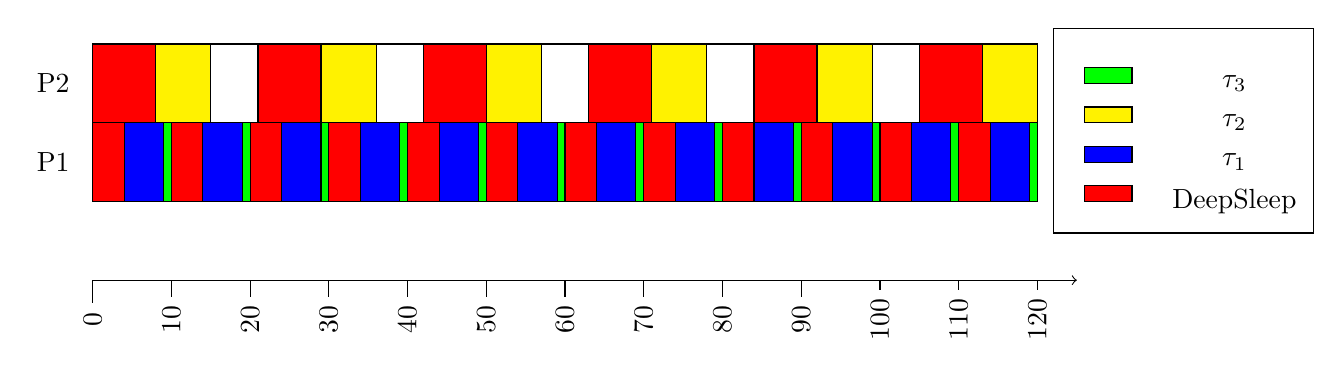
\begin{tikzpicture}
\node at (-0.5,0.5) {P1};
\node at (-0.5,1.5) {P2};
%P1 DS
\draw[fill=red] (0,0) rectangle (0.4,1) ;
\draw[fill=red] (1,0) rectangle (1.4,1) ;
\draw[fill=red] (2,0) rectangle (2.4,1) ;
\draw[fill=red] (3,0) rectangle (3.4,1) ;
\draw[fill=red] (4,0) rectangle (4.4,1) ;
\draw[fill=red] (5,0) rectangle (5.4,1) ;
\draw[fill=red] (6,0) rectangle (6.4,1) ;
\draw[fill=red] (7,0) rectangle (7.4,1) ;
\draw[fill=red] (8,0) rectangle (8.4,1) ;
\draw[fill=red] (9,0) rectangle (9.4,1) ;
\draw[fill=red] (10,0) rectangle (10.4,1) ;
\draw[fill=red] (11,0) rectangle (11.4,1) ;
%P1 T1
\draw[fill=blue] (0.4,0) rectangle (0.9,1) ;
\draw[fill=blue] (1.4,0) rectangle (1.9,1) ;
\draw[fill=blue] (2.4,0) rectangle (2.9,1) ;
\draw[fill=blue] (3.4,0) rectangle (3.9,1) ;
\draw[fill=blue] (4.4,0) rectangle (4.9,1) ;
\draw[fill=blue] (5.4,0) rectangle (5.9,1) ;
\draw[fill=blue] (6.4,0) rectangle (6.9,1) ;
\draw[fill=blue] (7.4,0) rectangle (7.9,1) ;
\draw[fill=blue] (8.4,0) rectangle (8.9,1) ;
\draw[fill=blue] (9.4,0) rectangle (9.9,1) ;
\draw[fill=blue] (10.4,0) rectangle (10.9,1) ;
\draw[fill=blue] (11.4,0) rectangle (11.9,1) ;
%P1 T3
\draw[fill=green] (0.9,0) rectangle (1,1) ;
\draw[fill=green] (1.9,0) rectangle (2,1) ;
\draw[fill=green] (2.9,0) rectangle (3,1) ;
\draw[fill=green] (3.9,0) rectangle (4,1) ;
\draw[fill=green] (4.9,0) rectangle (5,1) ;
\draw[fill=green] (5.9,0) rectangle (6,1) ;
\draw[fill=green] (6.9,0) rectangle (7,1) ;
\draw[fill=green] (7.9,0) rectangle (8,1) ;
\draw[fill=green] (8.9,0) rectangle (9,1) ;
\draw[fill=green] (9.9,0) rectangle (10,1) ;
\draw[fill=green] (10.9,0) rectangle (11,1) ;
\draw[fill=green] (11.9,0) rectangle (12,1) ;

\draw[fill=red] (0.0,1) rectangle (0.8,2) ;
\draw[fill=yellow] (0.8,1) rectangle (1.5,2) ;
\draw[fill=white] (1.5,1) rectangle (2.1,2) ;

\draw[fill=red] (2.1,1) rectangle (2.899999904632568,2) ;
\draw[fill=yellow] (2.899999904632568,1) rectangle (3.5999999046325684,2) ;
\draw[fill=white] (3.5999999046325684,1) rectangle (4.199999904632568,2) ;

\draw[fill=red] (4.2,1) rectangle (4.9999998092651365,2) ;
\draw[fill=yellow] (4.9999998092651365,1) rectangle (5.699999809265137,2) ;
\draw[fill=white] (5.699999809265137,1) rectangle (6.299999809265136,2) ;

\draw[fill=red] (6.2999997,1) rectangle (7.099999713897705,2) ;
\draw[fill=yellow] (7.099999713897705,1) rectangle (7.799999713897705,2) ;
\draw[fill=white] (7.799999713897705,1) rectangle (8.399999713897705,2) ;

\draw[fill=red] (8.4,1) rectangle (9.199999618530274,2) ;
\draw[fill=yellow] (9.199999618530274,1) rectangle (9.899999618530273,2) ;
\draw[fill=white] (9.899999618530273,1) rectangle (10.499999618530273,2) ;

\draw[fill=red] (10.5,1) rectangle (11.3,2) ;
\draw[fill=yellow] (11.3,1) rectangle (12.0,2) ;

\draw [->](0,-1) -- coordinate (x axis mid) (12.5,-1);
\draw (0,-1) -- (0,-1.5) node[fill=white,rotate=90] {0};
\draw (1,-1) -- (1,-1.5) node[fill=white,rotate=90] {10};
\draw (2,-1) -- (2,-1.5) node[fill=white,rotate=90] {20};
\draw (3,-1) -- (3,-1.5) node[fill=white,rotate=90] {30};
\draw (4,-1) -- (4,-1.5) node[fill=white,rotate=90] {40};
\draw (5,-1) -- (5,-1.5) node[fill=white,rotate=90] {50};
\draw (6,-1) -- (6,-1.5) node[fill=white,rotate=90] {60};
\draw (7,-1) -- (7,-1.5) node[fill=white,rotate=90] {70};
\draw (8,-1) -- (8,-1.5) node[fill=white,rotate=90] {80};
\draw (9,-1) -- (9,-1.5) node[fill=white,rotate=90] {90};
\draw (10,-1) -- (10,-1.5) node[fill=white,rotate=90] {100};
\draw (11,-1) -- (11,-1.5) node[fill=white,rotate=90] {110};
\draw (12,-1) -- (12,-1.5) node[fill=white,rotate=90] {120};

\draw[fill=white] (12.2,-0.4) rectangle (15.5,2.2) ;
\draw[fill=red] (12.6,0) rectangle (13.2,0.2) ;
\draw (14.5,0) -- (14.5,0) node[fill=white] {DeepSleep};
\draw[fill=blue] (12.6,0.5) rectangle (13.2,0.7) ;
\draw (14.5,0.5) -- (14.5,0.5) node[fill=white] {$\tau_1$};
\draw[fill=yellow] (12.6,1) rectangle (13.2,1.2) ;
\draw (14.5,1) -- (14.5,1) node[fill=white] {$\tau_2$};
\draw[fill=green] (12.6,1.5) rectangle (13.2,1.7) ;
\draw (14.5,1.5) -- (14.5,1.5) node[fill=white] {$\tau_3$};
\end{tikzpicture}}
\end{center}
\caption{Insertion locale de tâches d'endormissements dans un multiprocesseur} \label{fig:dmmpl}
\end{figure}
\begin{figure}[!h]
\begin{center}
\resizebox{15cm}{4cm}{
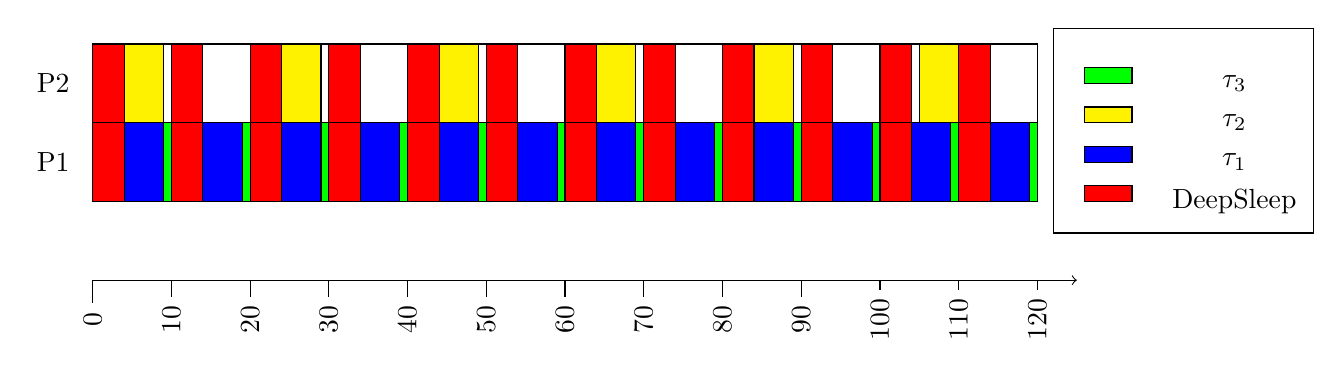
\begin{tikzpicture}
\node at (-0.5,0.5) {P1};
\node at (-0.5,1.5) {P2};
%P1 DS
\draw[fill=red] (0,0) rectangle (0.4,1) ;
\draw[fill=red] (1,0) rectangle (1.4,1) ;
\draw[fill=red] (2,0) rectangle (2.4,1) ;
\draw[fill=red] (3,0) rectangle (3.4,1) ;
\draw[fill=red] (4,0) rectangle (4.4,1) ;
\draw[fill=red] (5,0) rectangle (5.4,1) ;
\draw[fill=red] (6,0) rectangle (6.4,1) ;
\draw[fill=red] (7,0) rectangle (7.4,1) ;
\draw[fill=red] (8,0) rectangle (8.4,1) ;
\draw[fill=red] (9,0) rectangle (9.4,1) ;
\draw[fill=red] (10,0) rectangle (10.4,1) ;
\draw[fill=red] (11,0) rectangle (11.4,1) ;
%P1 T1
\draw[fill=blue] (0.4,0) rectangle (0.9,1) ;
\draw[fill=blue] (1.4,0) rectangle (1.9,1) ;
\draw[fill=blue] (2.4,0) rectangle (2.9,1) ;
\draw[fill=blue] (3.4,0) rectangle (3.9,1) ;
\draw[fill=blue] (4.4,0) rectangle (4.9,1) ;
\draw[fill=blue] (5.4,0) rectangle (5.9,1) ;
\draw[fill=blue] (6.4,0) rectangle (6.9,1) ;
\draw[fill=blue] (7.4,0) rectangle (7.9,1) ;
\draw[fill=blue] (8.4,0) rectangle (8.9,1) ;
\draw[fill=blue] (9.4,0) rectangle (9.9,1) ;
\draw[fill=blue] (10.4,0) rectangle (10.9,1) ;
\draw[fill=blue] (11.4,0) rectangle (11.9,1) ;
%P1 T3
\draw[fill=green] (0.9,0) rectangle (1,1) ;
\draw[fill=green] (1.9,0) rectangle (2,1) ;
\draw[fill=green] (2.9,0) rectangle (3,1) ;
\draw[fill=green] (3.9,0) rectangle (4,1) ;
\draw[fill=green] (4.9,0) rectangle (5,1) ;
\draw[fill=green] (5.9,0) rectangle (6,1) ;
\draw[fill=green] (6.9,0) rectangle (7,1) ;
\draw[fill=green] (7.9,0) rectangle (8,1) ;
\draw[fill=green] (8.9,0) rectangle (9,1) ;
\draw[fill=green] (9.9,0) rectangle (10,1) ;
\draw[fill=green] (10.9,0) rectangle (11,1) ;
\draw[fill=green] (11.9,0) rectangle (12,1) ;

\draw[fill=white] (0,1) rectangle (12,2) ;
\draw[fill=red] (0,1) rectangle (0.4,2) ;
\draw[fill=red] (1,1) rectangle (1.4,2) ;
\draw[fill=red] (2,1) rectangle (2.4,2) ;
\draw[fill=red] (3,1) rectangle (3.4,2) ;
\draw[fill=red] (4,1) rectangle (4.4,2) ;
\draw[fill=red] (5,1) rectangle (5.4,2) ;
\draw[fill=red] (6,1) rectangle (6.4,2) ;
\draw[fill=red] (7,1) rectangle (7.4,2) ;
\draw[fill=red] (8,1) rectangle (8.4,2) ;
\draw[fill=red] (9,1) rectangle (9.4,2) ;
\draw[fill=red] (10,1) rectangle (10.4,2) ;
\draw[fill=red] (11,1) rectangle (11.4,2) ;

\draw[fill=yellow] (0.4,1) rectangle (0.9,2) ;
\draw[fill=yellow] (2.4,1) rectangle (2.9,2) ;
\draw[fill=yellow] (4.4,1) rectangle (4.9,2) ;
\draw[fill=yellow] (6.4,1) rectangle (6.9,2) ;
\draw[fill=yellow] (8.4,1) rectangle (8.9,2) ;
\draw[fill=yellow] (10.5,1) rectangle (11,2) ;

\draw [->](0,-1) -- coordinate (x axis mid) (12.5,-1);
\draw (0,-1) -- (0,-1.5) node[fill=white,rotate=90] {0};
\draw (1,-1) -- (1,-1.5) node[fill=white,rotate=90] {10};
\draw (2,-1) -- (2,-1.5) node[fill=white,rotate=90] {20};
\draw (3,-1) -- (3,-1.5) node[fill=white,rotate=90] {30};
\draw (4,-1) -- (4,-1.5) node[fill=white,rotate=90] {40};
\draw (5,-1) -- (5,-1.5) node[fill=white,rotate=90] {50};
\draw (6,-1) -- (6,-1.5) node[fill=white,rotate=90] {60};
\draw (7,-1) -- (7,-1.5) node[fill=white,rotate=90] {70};
\draw (8,-1) -- (8,-1.5) node[fill=white,rotate=90] {80};
\draw (9,-1) -- (9,-1.5) node[fill=white,rotate=90] {90};
\draw (10,-1) -- (10,-1.5) node[fill=white,rotate=90] {100};
\draw (11,-1) -- (11,-1.5) node[fill=white,rotate=90] {110};
\draw (12,-1) -- (12,-1.5) node[fill=white,rotate=90] {120};

\draw[fill=white] (12.2,-0.4) rectangle (15.5,2.2) ;
\draw[fill=red] (12.6,0) rectangle (13.2,0.2) ;
\draw (14.5,0) -- (14.5,0) node[fill=white] {DeepSleep};
\draw[fill=blue] (12.6,0.5) rectangle (13.2,0.7) ;
\draw (14.5,0.5) -- (14.5,0.5) node[fill=white] {$\tau_1$};
\draw[fill=yellow] (12.6,1) rectangle (13.2,1.2) ;
\draw (14.5,1) -- (14.5,1) node[fill=white] {$\tau_2$};
\draw[fill=green] (12.6,1.5) rectangle (13.2,1.7) ;
\draw (14.5,1.5) -- (14.5,1.5) node[fill=white] {$\tau_3$};
\end{tikzpicture}}
\end{center}
\caption{Insertion globale de tâches d'endormissements dans un multiprocesseur} \label{fig:dmmpg}
\end{figure}
